\begin{frame}
	\begin{minipage}[t][0.6\textheight][t]{\textwidth}
		\begin{columns}
			\column{0.5\textwidth}
			\begin{overlayarea}{\textwidth}{\textheight}
				\only<1->{\myheading{Better Regularization}}
				\justify
				\only<1>{\textbf{Dropout:} A Simple Way to Prevent Neural Networks from Overfitting \cite{DBLP:journals/corr/abs-1207-0580} }
				\only<2>{ \textbf{Batch Normalization:} Acts as a regularizer in some cases \cite{DBLP:conf/icml/IoffeS15})
				}
			\end{overlayarea}
			\column{0.5\textwidth}
			\begin{overlayarea}{\textwidth}{\textheight}
				\begin{figure}
					\centering
					\only<1>{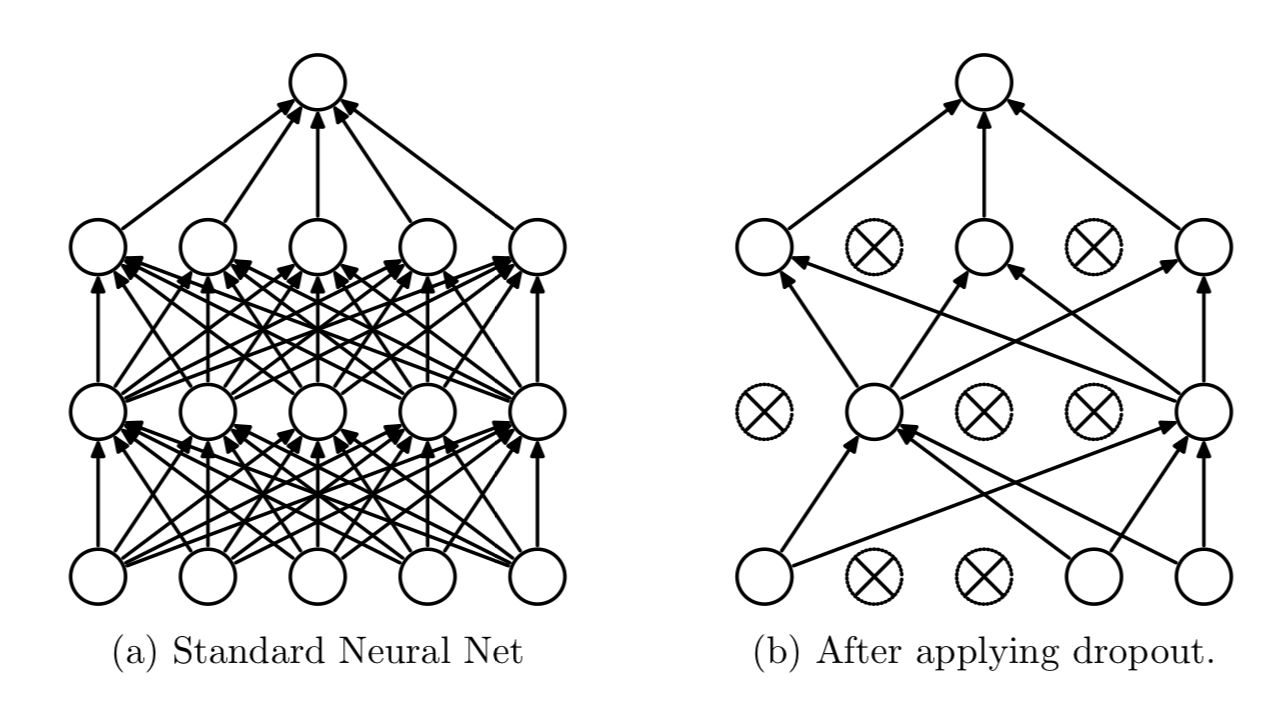
\includegraphics[scale=0.3]{images/module5/dropout}}
					\only<2>{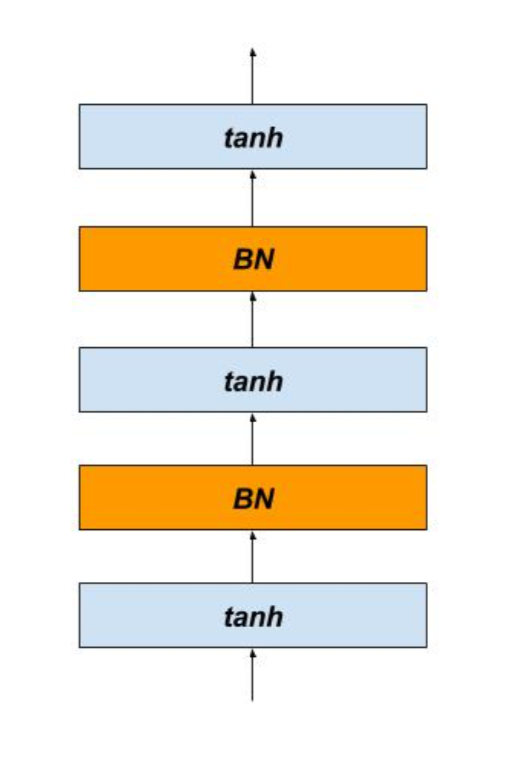
\includegraphics[scale=0.4]{images/module5/batch_norm}}
				\end{figure}
			\end{overlayarea}
		\end{columns}
	\end{minipage}
	\begin{minipage}[t][0.4\textheight][t]{\textwidth}
		\begin{overlayarea}{\textwidth}{\textheight}
			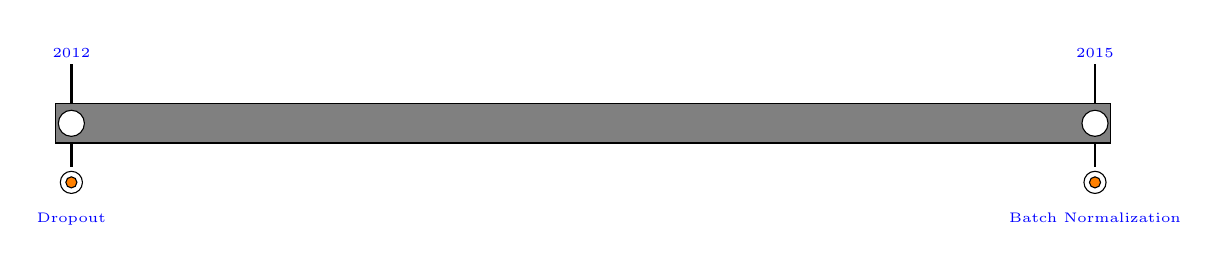
\begin{tikzpicture}[datemarker/.style={circle, draw=black,fill=white},textlabel/.style={anchor=center,text height=1.7ex,text depth=.25ex}]
				\tikzset{every node/.style={font=\tiny, color=blue}}\draw[fill=gray](-0.2,0) rectangle (13.2,0.5) node[white, below]{};
				\onslide<1->{\node at (0.0, 0.25) [datemarker] {};}
				\onslide<1->{\draw [line width=1pt] (0.0, 0.5) to (0.0, 1.0);}
				\onslide<1->{\draw (0.0, 1.2) node [textlabel]{2012};}
				\onslide<1->{\draw [fill=orange](0.0, -0.5) circle (2pt){};}
				\onslide<1->{\draw(0.0, -0.5) circle (4pt){};}
				\onslide<1->{\draw [line width=1pt] (0.0, 0) to (0.0, -0.3);}
				\onslide<1->{\draw (0.0,-0.9) node [textlabel] {Dropout};}
				\onslide<2->{\node at (13.0, 0.25) [datemarker] {};}
				\onslide<2->{\draw [line width=1pt] (13.0, 0.5) to (13.0, 1.0);}
				\onslide<2->{\draw (13.0, 1.2) node [textlabel]{2015};}
				\onslide<2->{\draw [fill=orange](13.0, -0.5) circle (2pt){};}
				\onslide<2->{\draw(13.0, -0.5) circle (4pt){};}
				\onslide<2->{\draw [line width=1pt] (13.0, 0) to (13.0, -0.3);}
				\onslide<2->{\draw (13.0,-0.9) node [textlabel] {Batch Normalization};}
			\end{tikzpicture}
		\end{overlayarea}
	\end{minipage}
\end{frame}
